\label{sec:L1}

\subsection{$l_1$ norm}

A more formal approach convexifies $(1)$ by replacing the $l_0$ norm with an $l_1$ norm:
\begin{equation}
 \label{eq:L1 modeling}
 \alpha_{x} = \arg\min_{\alpha}||\alpha||_1, s.t. ||x-\mathbf{D}\alpha||_2 \le \varepsilon
\end{equation}
This can be cast as a linear Programming(LP) problem, for which solutions are available even in large-scale problems, owing to modern interior-point linear programming methods. This approach to overcomplete signal representation was called Basis-Pursuit(BP)\cite{chen1998atomic}, which observed that it sometimes gave highly sparse solutions to problems known to have such solutions, and showed that it could, in specific cases, outperform the greedy Matching Pursuit approach in generating sparse solutions.

Considering these advantages, $l_1$ norm comprises a large proportion of sparse representation in geometry processing.

\paragraph{Reconstruction}In recent years, many robust surface reconstruction techniques have been developed that can deal with a variety of acquisition errors like noise, outliers, missing data(holes) or registration artifacts. They are commonly based on a robust $l_1$ optimization approach and are able to produce high-quality output despite very difficult data.

Actually, the idea of $l_1$ optimization has a long history. Decades ago, \cite{weber1909theory} had proposed the optimal location problem which is a statistical tool that is traditionally applied globally to multivariate non-parametric point-samples to generate a good representative for a large number of samples in the presence of noise and outliers. This problem is known as $l_1$ median\cite{brown1983statistical,small1990survey} in statistic finding a robust global center of an arbitrary set of points.

\cite{lipman2007parameterization} applies this tool locally in a geometric context and introduces a parameterization-free local projection operator(LOP) which does not rely on estimating a local normal. LOP robustly fits a set of resampling points to a noisy point cloud((a) in Figure...) by iteratively applying a system attractive forces defined by the input points and is particulary attractive for reconstruction since it does not put many constraints on the nature of the input data, i.e., it does not require a well-defined surface parameterization nor a surface which can be locally well approximated with a plane. But LOP is subject to a local density parameter, i.e., the result is affected by the points distributions.

Considering the limitation of LOP for non-uniform distributions common in raw data, a weighted LOP(WLOP) by modifying and extending LOP operator in \cite{huang2009consolidation} which is a two phase method focusing on reliable normal estimation to consolidate an unorganized point cloud is proposed. Actually, it is just a preprocess of the input point cloud((b) in Figure...). By taking into account a local density measure, WLOP is first used to produce a set of denoised, outlier-free and evenly distributed points to improve the reliability of local PCA for initialization of normals which are used in the following normal estimation phase. But it lacks of theoretic guarantee and cannot address the missing data problem like LOP.

In fact, LOP requires high computational effort due to the nature of $l_1$ optimization. To improve efficiency, \cite{preiner2014CPF} presents a novel continuous formulation of the WLOP operator based on a Gaussian mixture describing the input point density to make a robust reconstruction at interactive frame rates for moderately sized dynamic point sets possible((c) in Figure...).

In addition to these $l_1$ median based works mentioned above, \cite{avron2010L1} introduces an $l_1$ sparse method decoupling orientations and positions for the reconstruction of a piecewise smooth point set surface with sharp feature((d) in Figure...). They first solve for the point orientations and then, based on the piecewise smooth normals, solve for the point positions. Both problems are formulated in a similar $l_1$ nature, yielding a consistent solution.

Figure...shows all the reconstruction results of these methods.

\begin{figure}[ht]
  \centering
  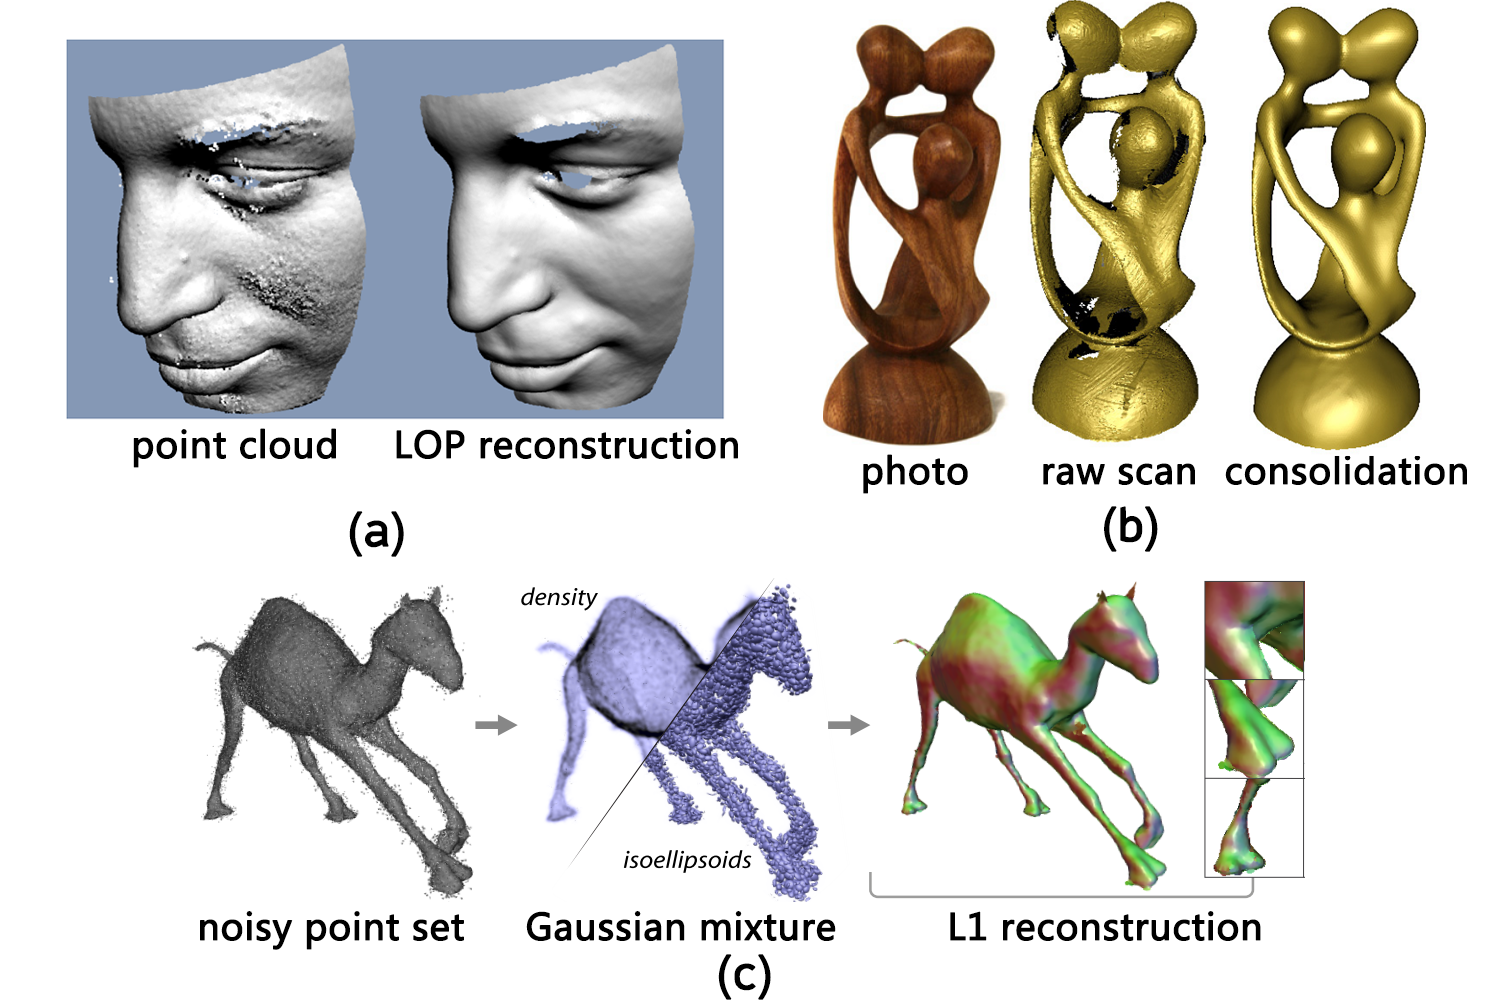
\includegraphics[width=3in]{images/reconstruction_L1}
  \caption{$l_1$ optimization: reconstruction results. (a): \cite{lipman2007parameterization}. (b): \cite{huang2009consolidation}. (c): \cite{preiner2014CPF}. (d): \cite{avron2010L1}.}
\end{figure}

\paragraph{Skeleton extraction}Skeletal shape representations have been intensely studied in various fields and utilized in a variety of applications for shape modeling and analysis. \cite{huang2013l1} finds out a new application for $l_1$ median, they introduce $l_1$-medial skeleton as a curve skeleton representation for 3D point cloud data(Figure...). Without building any point connectivity or estimating point normals, they directly project point samples onto their local centers as $l_1$ medians with growing neighborhood and push the projected samples via conditional regularization to obtain a uniform distribution of samples along skeleton branches. It is a simple but powerful approach for extracting skeletons from unorganized, unoriented and incomplete 3D raw point clouds.

\begin{figure}[ht]
  \centering
  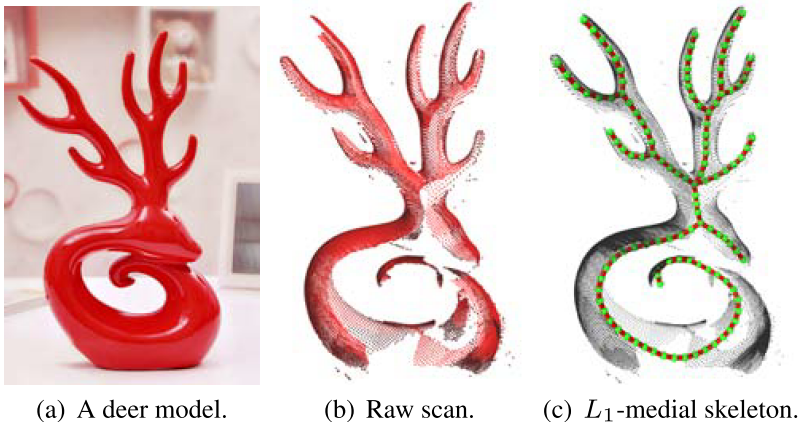
\includegraphics[width=3in]{images/skeleton_L1}
  \caption{$l_1$ optimization: skeleton extraction\cite{huang2013l1}. Given an unorganized, unoriented, and incomplete raw scan with noise and outliers, a complete and quality curve skeleton is extracted.}
\end{figure}

\paragraph{Mesh Denoising} Like \cite{he2013mesh} mentioned above, most previous methods rely on computation of differential properties to detect noise which is unreliable and unstable and require the user to carefully tune the model parameters case by case and rarely have theoretical guarantees. To address these problems, \cite{wang2014decoupling} presents a two phase approach for decoupling features and noise on discrete surfaces. After generating a base mesh which is obtained by denoising the input data using a global Laplacian regularization smoothing optimization in which the smoothness parameter is automatically chosen by adopting the generalized cross-validation scheme, sharp features are extracted from the residual between base mesh and input mesh based on an $l_1$ analysis compressed sensing optimization. It is achieved by the discovery that sharp features can be sparsely represented in some coherent dictionary which is constructed by the pseudo-inverse matrix of the Laplacian of the shape, Figure... gives the 1D illustration and the denoising results. It is the first time noise and features are analyzed and separated in such an elegant manner with guarantees by statistical theory.

\begin{figure}[ht]
  \centering
  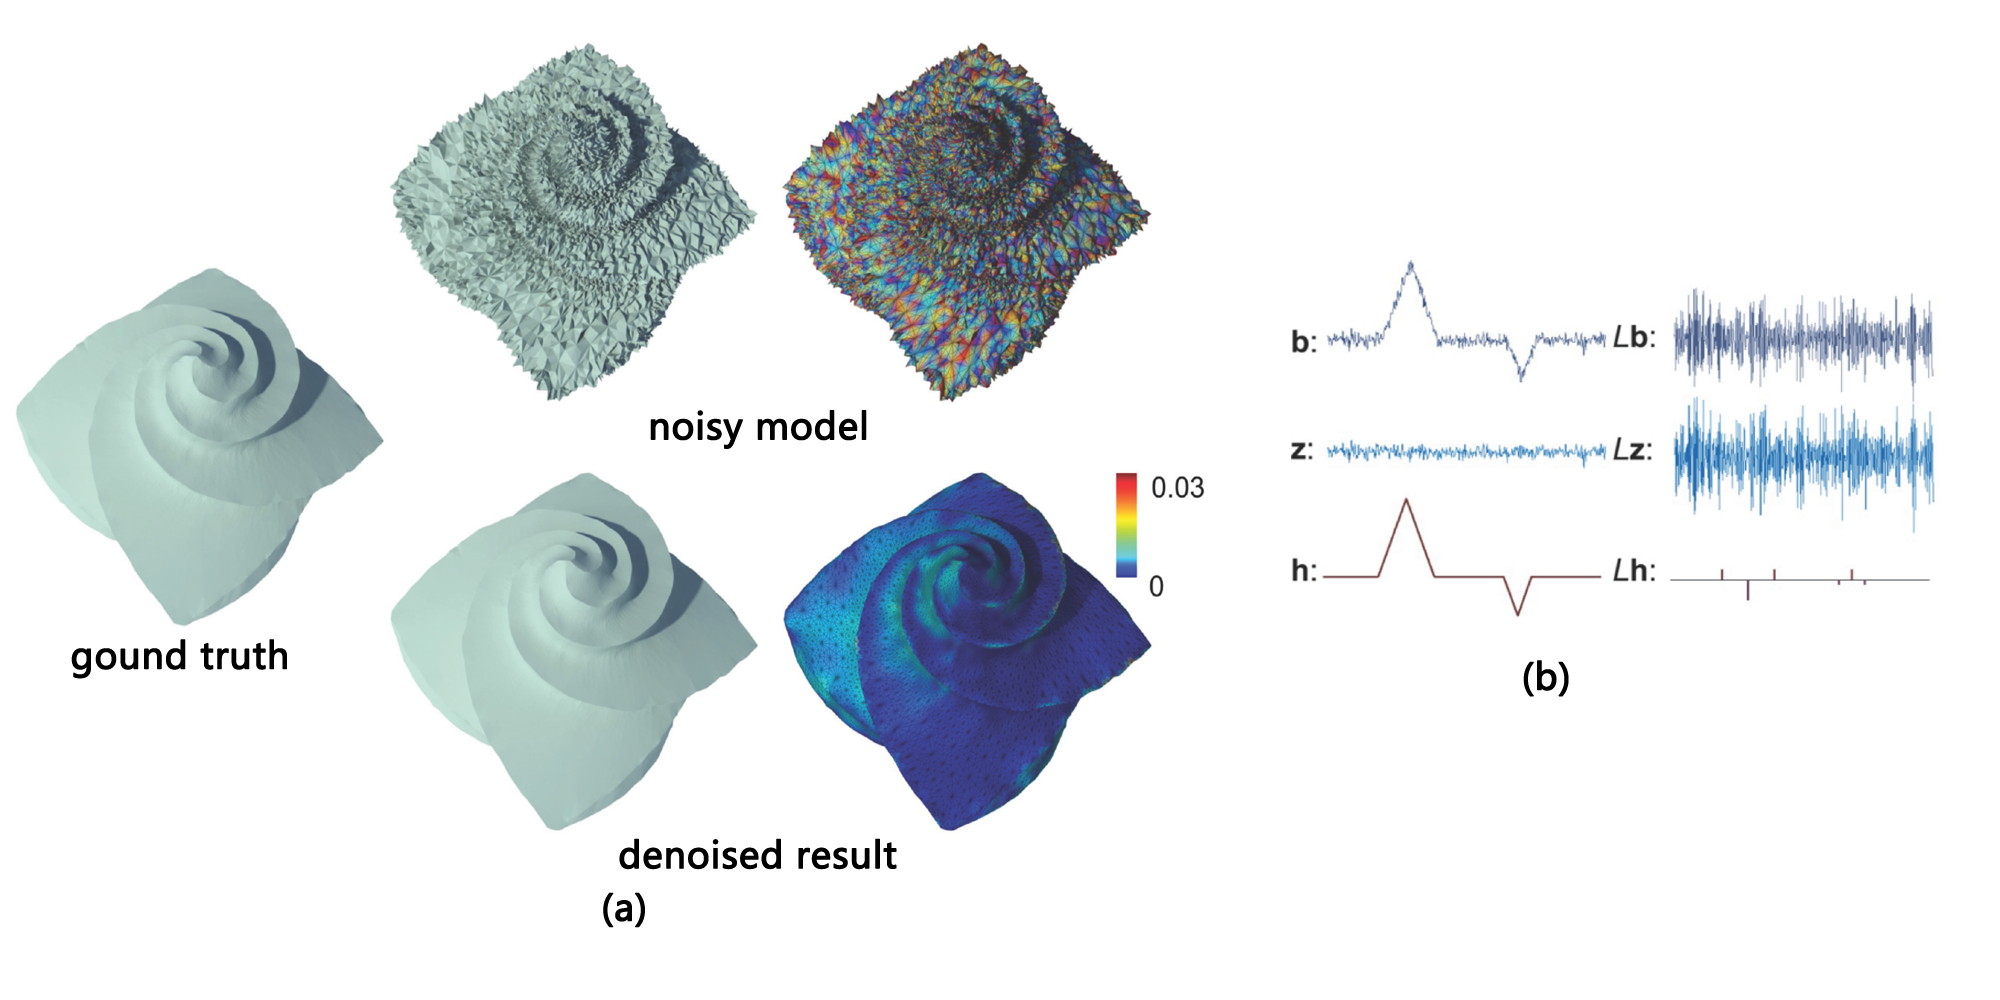
\includegraphics[width=3in]{images/denoise_L1}
  \caption{$l_1$ optimization: mesh denoising\cite{wang2014decoupling}. (a) is a denoising example. (b) is the 1D illustration of signals and their Laplacians. Left:the residual $\mathbf{b}$ (upper) is a mixture of noise $\mathbf{z}$(middle) and features $\mathbf{h}$(lower). Right: the corresponding Laplacians of signals on the left.}
\end{figure}

\paragraph{Shape Matching} Matching of deformable shapes is a notoriously difficult problem playing an important role in many application, non-rigid matching typically uses point-wise representation of correspondence, which results in the number of degrees of freedom growing exponentially with the number of matched points. \cite{pokrass2013sparse} poses the problem of finding intrinsic correspondence between near-isometric deformable shapes as a permuted sparse modeling. It is based on the observation that choosing the discretized eigenfunctions of the Laplace-Beltrami operator of two shapes will cause the low-distortion correspondence being represented by a nearly diagonal, and therefore very sparse matrix, and among other dense correspondence techniques, this method relies on the smallest amount of information. Figure...

\begin{figure}[ht]
  \centering
  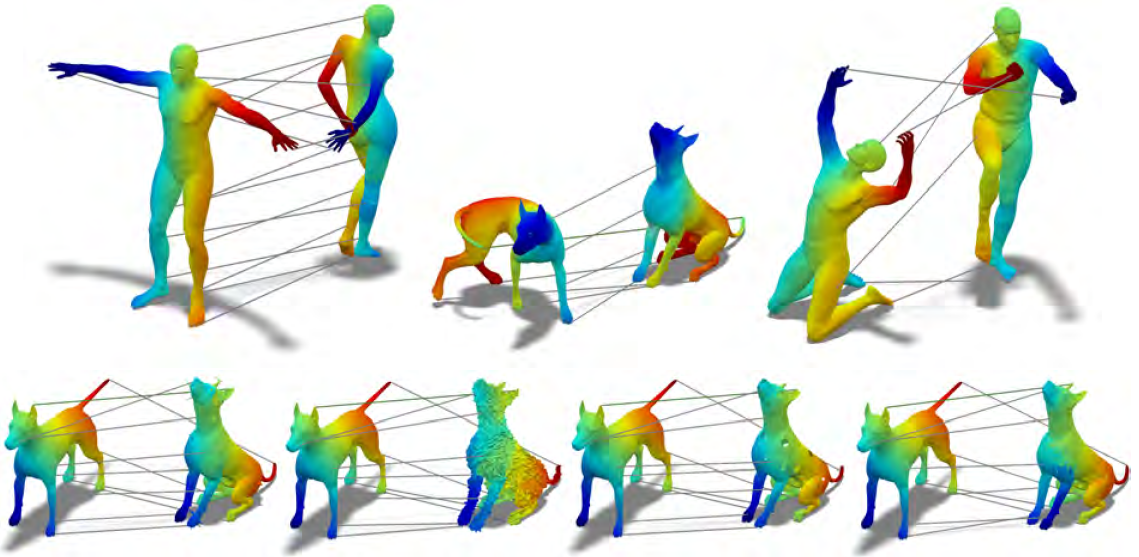
\includegraphics[width=3in]{images/matching_L1}
  \caption{$l_1$ optimization: shape matching\cite{wang2014decoupling}. First row: point-to-point correspondences between different non-isometric shapes. Second row: point-to-point correspondence between SHREC shapes undergoing nearly isometric deformations and noise.}
\end{figure}

\paragraph{Barycentric coordinates}

\begin{figure}[ht]
  \centering
  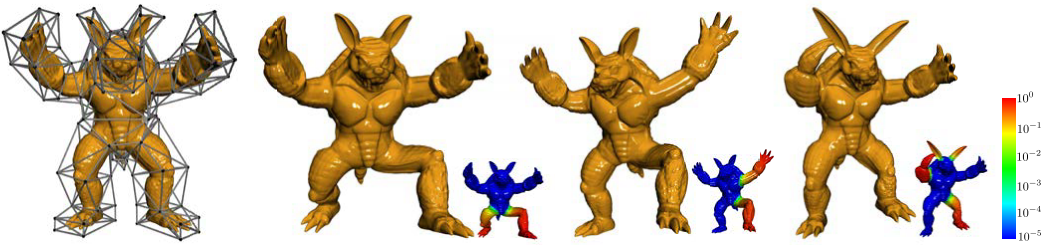
\includegraphics[width=3in]{images/LBC_L1}
  \caption{$l_1$ optimization: local barycentric coordinates\cite{}. Using LBC for 3D cage-based manipulation allows for local, smooth and shape-aware deformations. Only parts near the manipulated control points are deformed, as indicated by the color-coding.}
\end{figure}

In summary, many robust surface reconstruction techniques have been developed to deal with a variety of acquisition errors like noise, outliers, missing data(holes) or registration artifacts. They are commonly based on a robust $l_1$ optimization approach and are able to produce high-quality output despite very difficult data. Though typical $l_1$ norm problems aim at reconstructing sparse signals from a large amount of measurement. It has also been applied to some other problems like polycube, correspondence and denoising mentioned above. Most of the $l_1$ techniques are typically too expensive to achieve interactive reconstruction times for at least moderately sized point sets, even for parallel implementations. Even though they are designed for quality rather than performance due to their nature, the performance problem is worth researching. 